\section{Per-Cube Mesh Extraction}
\label{sec:percube}

\begin{figure*}[t]
  \centering
  \begin{subfigure}[b]{0.24\linewidth}
    \centering
    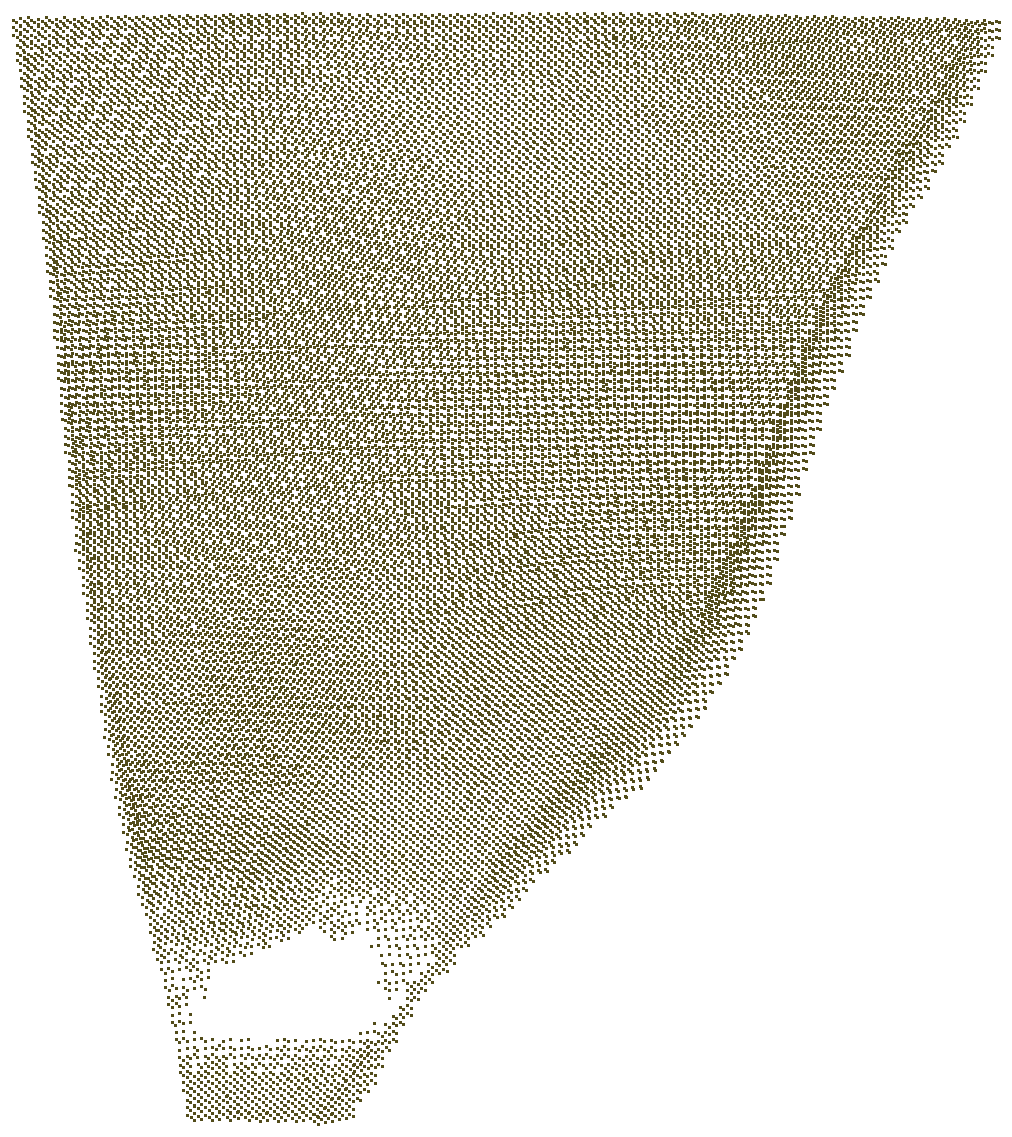
\includegraphics[width=\linewidth]{figures/overview00_crop.png}
    \caption{MLS-collapsed points}
  \end{subfigure}
  \hfill
  \begin{subfigure}[b]{0.24\linewidth}
    \centering
    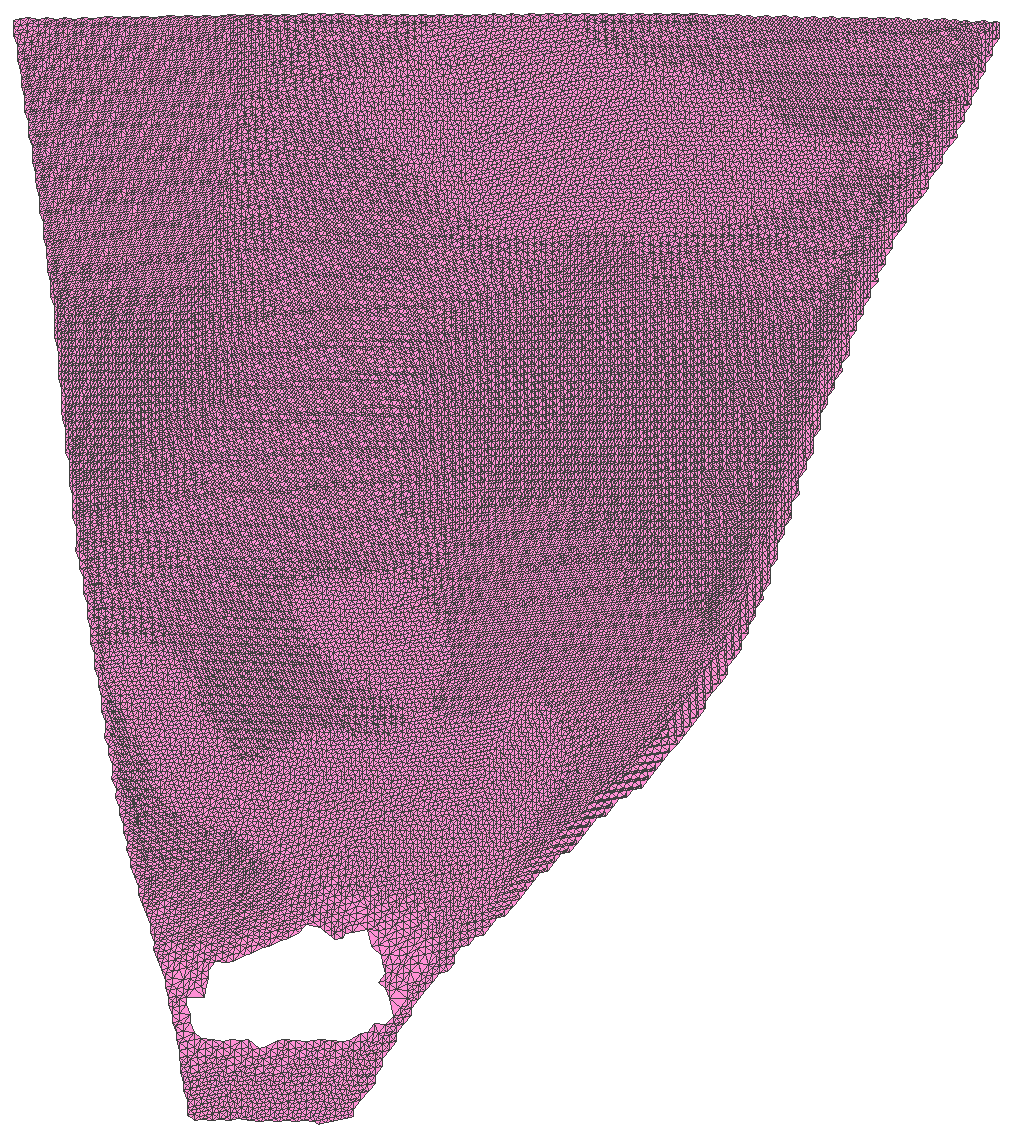
\includegraphics[width=\linewidth]{figures/overview01_crop.png}
    \caption{Guarded ball pivoting}
  \end{subfigure}
  \hfill
  \begin{subfigure}[b]{0.24\linewidth}
    \centering
    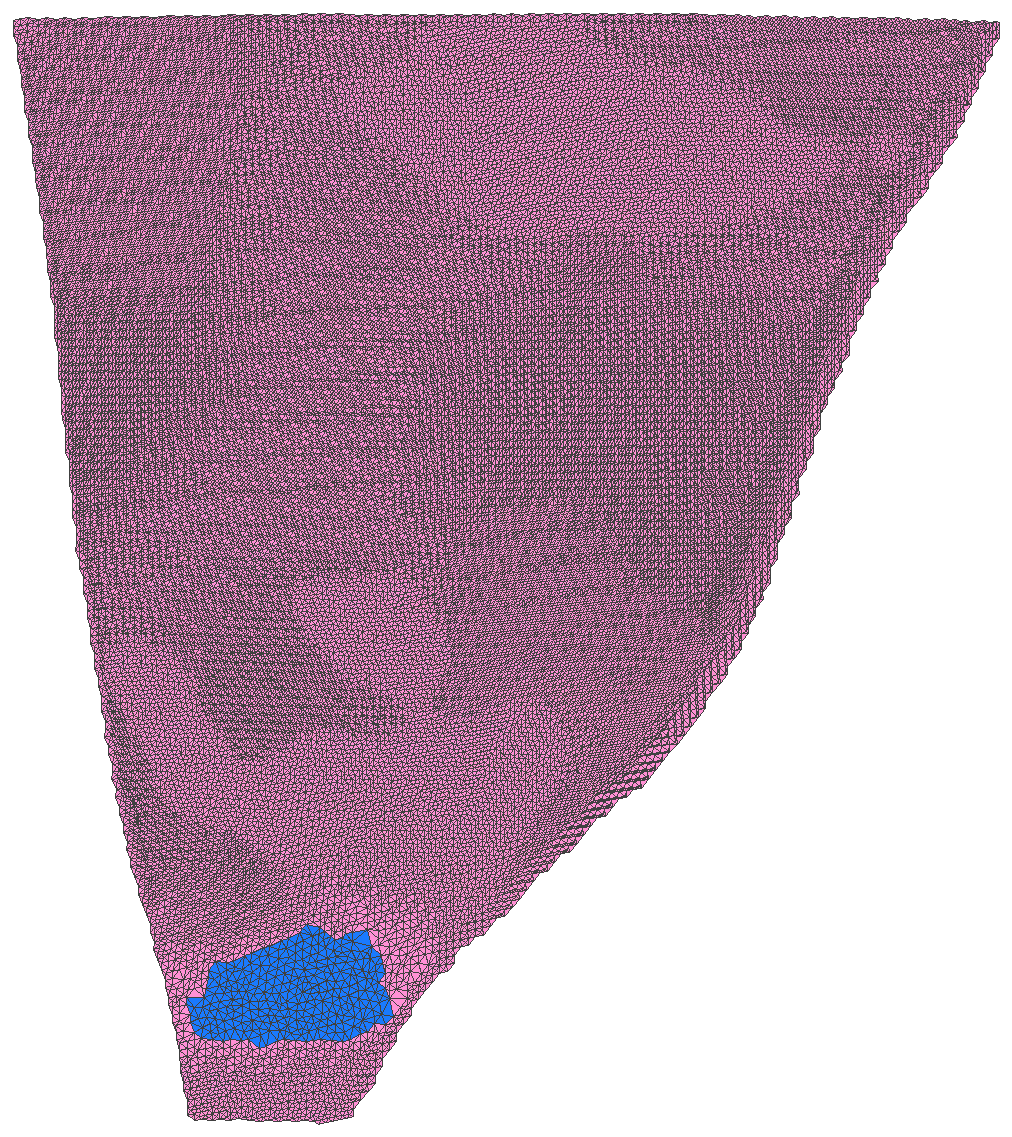
\includegraphics[width=\linewidth]{figures/overview02_crop.png}
    \caption{Interior loops filled (blue)}
  \end{subfigure}
  \hfill
  \begin{subfigure}[b]{0.24\linewidth}
    \centering
    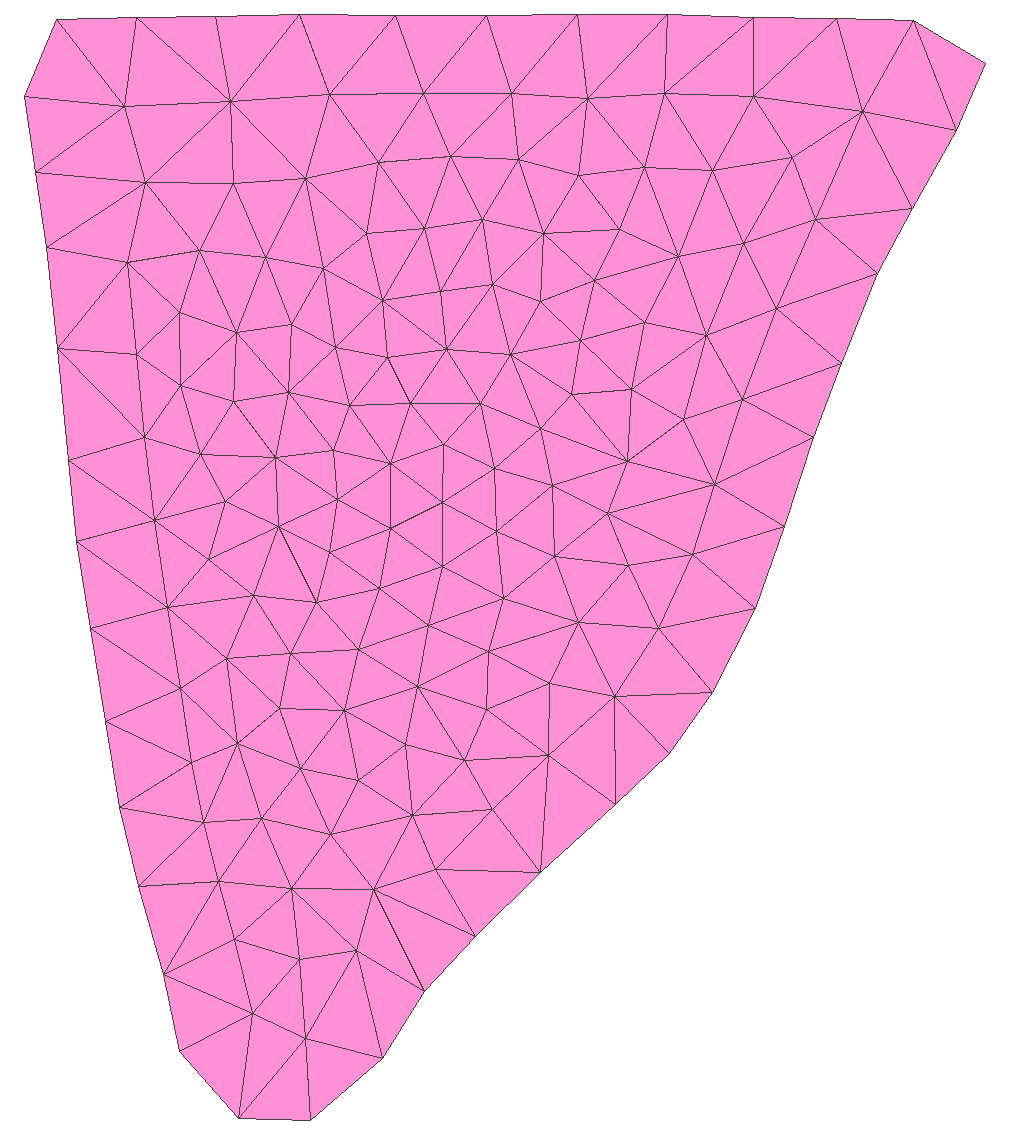
\includegraphics[width=\linewidth]{figures/overview03_crop.png}
    \caption{CVT/RVD remesh}
  \end{subfigure}
  \caption{The per-cube extraction stages on one PHerc0139 sheet. (a) Voxel-centre points after the iterated MLS projection has collapsed the several-voxel-thick prediction to a single sheet. (b) The consistently oriented, guard-gated ball-pivoting reconstruction; the remaining perforations are prediction gaps. (c) Clean interior loops are closed (filled regions shown in blue) while the genuine sheet boundary is left open. (d) The level-of-detail stage on the same sheet: the CVT/RVD remeshing of Section~\ref{sec:cvt} relocates samples into a near-isotropic blue-noise distribution.}
  \Description{Four panels showing the same roughly triangular papyrus sheet as a dotted point cloud, a dense pink triangle mesh with holes, the same mesh with blue filled patches, and a coarse triangulated version.}
  \label{fig:cube_stages}
\end{figure*}

Before meshing a cube we apply a lightweight input guard. A U-Net occasionally emits a degenerate prediction in which a region is filled as a solid block rather than a thin sheet; ball-pivoting cannot roll across a solid three-dimensional point fill, and meshing such a cube yields only fragmented debris. We detect these cubes by morphological erosion-survival: a small 3D erosion dissolves a genuine thin sheet entirely while a solid slab retains a large interior fraction. We additionally require that the surviving foreground form a solid filled rectangle across many consecutive slices, so that dense but legitimate wrap regions are never rejected. A cube that fails this guard is skipped and contributes nothing to the output rather than junk geometry.

We initialize our point cloud by extracting one point at the centre of each solid voxel of the input cube. Where the prediction is more than one voxel thick this yields a slab of points several voxels deep, so we first collapse and denoise it into a single clean sheet using an iterated moving least-squares (MLS) projection~\cite{levin2003mesh}: each point is moved along its local surface normal, estimated from a Wendland-weighted neighbourhood~\cite{wendland1995piecewise}, onto the local least-squares plane. Only the through-thickness component of this motion is non-zero, so the slab is thinned to a single sheet without the in-plane contraction we observed when we initially tried the closely-related locally optimal projection~\cite{lipman2007parameterization}. The projection itself is a standard tool; our observation is that choosing a projection method whose kernel has compact support makes the per-cube result consistent across cube boundaries, and that this boundary-consistency is precisely what makes our divide-and-conquer scroll meshing possible. Concretely, adjacent cubes are processed with an overlapping halo of shared input voxels, and because each projected position depends only on neighbours within a fixed radius, points in the shared region land in the same place in both cubes; the two cubes therefore present matching geometry to the welder. Finally, we trim the cloud so that the open mesh boundary falls inside the cube face, and weld points lying within 0.25 voxels of one another.

We then assign the point cloud a globally consistent normal orientation using the method of Hoppe et al. \shortcite{hoppe1992surface}, to ensure that all papyrus surfaces are consistently oriented as our algorithm requires. 

Meshing the point cloud requires an algorithm that is local (in order to join cubes together after processing); fast; and that is not designed to output a closed, watertight surface. We therefore use the ball-pivoting algorithm \cite{bernardini1999ball} (BPA), which we summarize as follows: three points form a triangle if a ball of a user specified radius $\rho$ touches them without containing any other point. Starting with a seed triangle, the ball pivots around each edge until it touches another point, forming a triangle. The process continues until all reachable edges have been tried, and then starts from another seed triangle until all points have been considered. We found that this simple approach satisfies our main criteria, at the cost of some small topological artifacts which are easily resolved (see below): it can be used to weld neighbouring cube surfaces into the complete scroll by setting the cube boundaries to the advancing front at the algorithm start, and it is very well-behaved on open surfaces. Our implementation of BPA includes several guards that keep the advancing front on a single sheet. A dihedral fold-back guard prevents the front from folding back over itself. A face-coherence guard rejects any candidate triangle whose normal turns too sharply away from the triangle that owns the pivot edge; without it, the ball tends to roll down onto an adjacent wrap instead of across a thin gap in its own sheet, stitching the two layers together. An anti-parallel guard similarly refuses to add a triangle that would bridge two oppositely-oriented surfaces lying close together, as occurs where neighbouring wraps nearly touch. A {\em wall guard} rejects candidates that are simultaneously steep against the local MLS normal and long: a fusion bridge stands nearly perpendicular to the sheet it fuses and must reach across the inter-wrap gap, whereas a genuine surface triangle is parallel to its vertex normals, so the conjunction fires only on through-thickness bridges and spares sharp folds. Finally, because a front can accumulate error gradually --- every individual pivot innocent while the front slowly climbs a through-thickness wall and gains whole turns --- each seed's growth carries a branch-cut-free integrated winding phase about the scroll axis, and a pivot whose accumulated phase leaves a tolerance band is refused; the surface beyond it is re-seeded as a distinct component. Guard thresholds appear in Appendix~\ref{app:terms}.

\paragraph{Quality-gated extraction.}
A smaller pivot radius can sometimes avoid a local fusion, but it can also discard surface coverage and explode the number of open boundary edges. We therefore do not tune $\rho$ by appearance. The adaptive controller begins at the normal radius and only tries smaller radii after a winding failure. A candidate is accepted only when it contains no abrupt full-turn edges or broad branch-local fusions, retains at least 95\% of the baseline point coverage, and introduces no more than 1.25 times the baseline boundary edges. If no candidate passes, the component is quarantined for cutting or an unverified downstream path. This makes the extraction decision part of the topology audit rather than an undocumented per-dataset parameter choice.

\subsection{Topological Cleanup}
\label{sec:cleanup}

A single voxel connected-component can hold several {\em disconnected} surface sheets that were projected and meshed together, because the moving least-squares projection operates on all of a component's points at once and nearby sheets pull on one another. Before anything else, we separate each meshed component into its connected pieces and re-project and re-mesh each one in isolation, this time from its {\em original} voxel-center points rather than from the already-projected vertices, so that the projection kernel sees only same-sheet neighbours and each sheet lands cleanly on its own surface. Re-projecting from the original points proves to be a reusable primitive, which we also apply after every split below to clean the ragged boundary a cut otherwise leaves behind.

At this stage, we may have multiple components erroneously attached in the same cube. This can be due either to proximity during the BPA algorithm, or more commonly due to errors in the input. As we now have meshes, we can detect these connections by finding every connected mesh component in the cube, and casting rays from each triangle centroid along its normal in both directions to determine if we should split the input geometry.

We categorize splits into two cases. First, we consider the case where one small bridge connects two levels of geometry; this is commonly caused by scroll NN prediction artifacts (Fig.~\ref{fig:bridgesplit}). We formulate finding these splits as a min-cut problem, and we solve it using the standard Edmonds-Karp algorithm. For more complex overlapping geometries, we use a lifted multicut solver \cite{keuper2015efficient} to solve an overlap reduction problem based on the formulation from Limper et al. \cite{limper2018box}. After splitting, each resulting piece is re-projected and re-meshed from its parent's original voxel points as described above, so that the new sheet boundaries come out clean rather than carrying the jagged trace of the cut.

\begin{figure*}[t]
  \centering
  \begin{subfigure}[b]{0.245\linewidth}
    \centering
    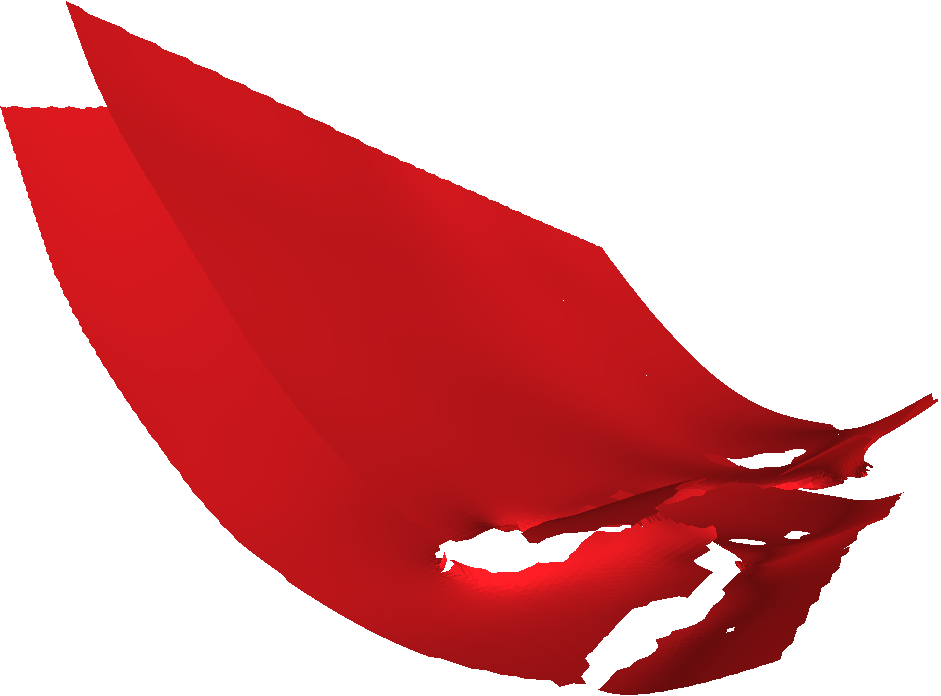
\includegraphics[width=\linewidth]{figures/neck_before00.png}
    \caption{Fused pair, before}
    \label{fig:bridgesplit_before}
  \end{subfigure}
  \hfill
  \begin{subfigure}[b]{0.245\linewidth}
    \centering
    
\includegraphics[width=\linewidth]{figures/neck_after01.png}
    \caption{Severed at the neck}
    \label{fig:bridgesplit_after}
  \end{subfigure}
  \hfill
  \begin{subfigure}[b]{0.245\linewidth}
    \centering
    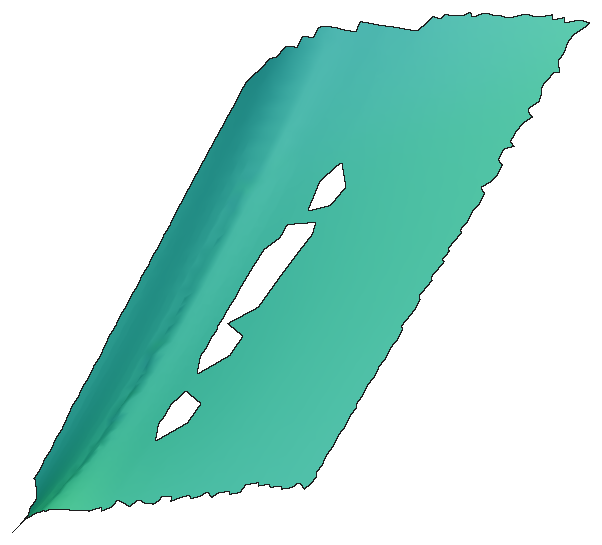
\includegraphics[width=\linewidth]{figures/holefill_before.png}
    \caption{Perforated sheet, before}
    \label{fig:holefill_before}
  \end{subfigure}
  \hfill
  \begin{subfigure}[b]{0.245\linewidth}
    \centering
    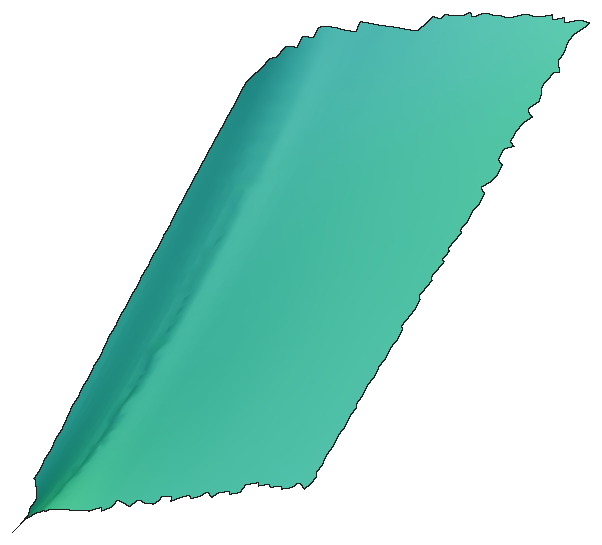
\includegraphics[width=\linewidth]{figures/holefill_after.png}
    \caption{Interior loops closed}
    \label{fig:holefill_after}
  \end{subfigure}
  \caption{The two mesh-space repairs that must happen before any parameterization is attempted, on real PHerc0139 cubes. (a,b) The U-Net has fused two sheets through a thin neck of bridge material; the bridge is detected and severed by min-cut, recovering two distinct sheets --- a fusion left in place would weld two wraps into one and make the winding topology unrecoverable. (c,d) Holes left by the ball-pivoting front and by gaps in the prediction are closed: exact three-edge loops directly, larger clean interior loops by constrained Delaunay with Liepa-style refinement~\cite{liepa2003filling}. Self-intersecting, non-manifold, or clearly exterior loops are rejected rather than force-filled, so a genuine sheet boundary is never sealed shut.}
  \Description{Four small panels: two mesh sheets joined by a thin bridge and then separated at it, followed by a perforated triangle mesh and the same mesh with its interior holes closed.}
  \label{fig:bridgesplit}
\end{figure*}

After each separation we split pinched vertex fans until every stage component is vertex-manifold. If holes are detected inside a component, we patch them at this stage (Fig.~\ref{fig:bridgesplit}c,d). Exact three-edge loops are closed directly. Other clean interior loops are projected to a local plane, triangulated by constrained Delaunay, and lifted back with Liepa-style refinement~\cite{liepa2003filling}; self-intersecting, non-manifold, or clearly exterior loops are rejected rather than force-filled.

Ball-pivoting can also fuse a sheet to itself without disconnecting it: where the advancing front rolls across a thin gap, it can close a loop that raises the sheet's genus into a small handle. Such handles are {\em non-separating}, so the cut-based splitters above, which sever {\em separating} necks, cannot remove them. After hole filling, we apply a tree--cotree decomposition and open every non-separating loop shorter than a fixed length bound by manifold-preserving vertex duplication. This reduces accidental local genus while leaving the long, scroll-scale cycles that represent genuine structure untouched.

\subsection{CVT/RVD Remeshing}
\label{sec:cvt}

Previous versions of ScrollFiesta used QEM for downsampling the ball-pivoting stage output. In practice, we found that this created numerous small sliver triangles and an uneven distribution of samples. We therefore perform level of detail using a centroidal Voronoi tessellation restricted to the reconstructed surface. We seed interior sites by area and boundary sites along every retained loop, then iterate the variational update of CWF~\cite{xu2024cwf}: each interior site solves a small fixed-cell system combining the ordinary centroidal (CVT) term with a normal-anisotropy term that pulls samples onto creases and thin features, with the CVT weight decaying across iterations (Appendix~\ref{app:terms}). Each updated site is projected back to the source surface, and the output triangles are the restricted-Delaunay dual of the restricted Voronoi diagram (RVD). Uniform density is used per cube at present. Unlike collapse-only QSlim/QEM, this operation relocates samples into a near-isotropic distribution, reduces slivers, and does not preserve a poor advancing-front tessellation merely because it arrived first.

Any component above the current size cap, an empty or invalid dual, or a result that fails the manifold checks falls back to the repaired QEM path; QEM can also be selected explicitly. The fallback rejects edge collapses or maintenance flips that would create an existing edge or reverse winding. Once remeshed, components with negligible area are removed as debris, and halo output is cut at the owned cube planes so that every geometric region has a single owner at assembly time.